\documentclass[9pt,table]{beamer} % options fleqn

\usepackage{/home/paul/Workspace/build/macros}


\usetheme[titleformat frame = smallcaps]{metropolis}
%\usepackage{FiraSans}
\usepackage{FiraMono}

\metroset{sectionpage=none}

%\usepackage[T1]{fontenc}


\setbeamersize{text margin left=5mm,text margin right=5mm} 
%\setbeamersize{text margin left=9mm,text margin right=3mm} 

\setbeamertemplate{section in toc}[sections numbered]

% algorithms
\usepackage[ruled,linesnumbered]{algorithm2e}
\SetKwInput{KwInput}{Input}
\SetKwInput{KwOutput}{Output}

% typography
\usepackage{soul}

\usepackage{caption}

\usepackage{varwidth}

\usepackage{dsfont}

% figures
\usepackage{svg}
%\svgpath{{figs/}}

% drawings
\usepackage{tikz}
\usetikzlibrary{shapes,shapes.misc,shapes.geometric}
\usetikzlibrary{positioning,fit,backgrounds}
\usetikzlibrary{trees,matrix}
\usetikzlibrary{decorations.pathreplacing,calligraphy}
%
\tikzset{cross/.style={cross out, draw=red, minimum size=3pt, line width=0.25mm, inner sep=0pt, outer sep=0pt}, cross/.default={1pt}}
%
\usepackage[skins,theorems]{tcolorbox}
\tcbset{highlight math style={colback=mLightBrown!20,colframe=black!2,sharp corners},bottom=2pt,top=2pt}
\tcbset{left skip={-.01\linewidth}, colback=mLightBrown!20,colframe=black!2,sharp corners,left=0pt,right=0pt}
%
\newcommand{\point}[1]{\textbf{\textcolor{mDarkTeal}{#1}}\quad}
%
%\definecolor{cobalt}{HTML}{0047AB}
\definecolor{aqua}{HTML}{00FFFF}
\newcommand{\kw}[1]{\textbf{\alert{#1}}}
\newcommand{\invsible}[1]{\textcolor{black!2}{#1}}
%
\definecolor{myteal}{rgb}{0.21, 0.46, 0.53}

\usepackage[position=bottom]{subfig}

\usepackage{tabularx}
\usepackage{booktabs}% http://ctan.org/pkg/booktabs
\newcommand{\tabitem}{\llap{\tiny$\blacksquare$}~~}

% handling lists
\usepackage{enumitem}

\usepackage{multimedia}

% tcolorbox
\usepackage[skins,theorems]{tcolorbox}
\tcbset{highlight math style={colback=mLightBrown!20,colframe=black!2,sharp corners},bottom=2pt,top=2pt}
\tcbset{left skip={-.01\linewidth}, colback=mLightBrown!20,colframe=black!2,sharp corners,left=0pt,right=0pt}


% references
\usepackage[backend=biber,style=authoryear]{biblatex}
%\usepackage[backend=biber,style=alphabetic]{biblatex}
\bibliography{/home/paul/Workspace/build/biblio}
\usepackage{bibentry}
\newcommand{\mycite}[2]{\footnotetext[#1]{\emph{\tiny{\citeauthor{#2},\,\citeyear{#2},}}\,\tiny{\citefield{#2}{title}}}}

%\renewcommand{\cite}[1]{\textcolor{myteal}{[\citeauthor{#1},\,\citeyear{#1}]}}%
%\newcommand{\mycite}[1]{\textcolor{myteal}{\cite{#1}}}%
\AtBeginEnvironment{frame}{\setcounter{footnote}{0}}

\usepackage{hyperref}


\graphicspath{{figs/}{examples/}{/home/paul/Workspace/data/standard_test_images}}




% add a sommaire
%\makeatletter
%\setbeamertemplate{headline}{%
%  \begin{beamercolorbox}[colsep=1.5pt]{upper separation line head}
%  \end{beamercolorbox}
%  \begin{beamercolorbox}{section in head/foot}
%    \vskip2pt\insertnavigation{\paperwidth}\vskip2pt
%  \end{beamercolorbox}%
%  \begin{beamercolorbox}[colsep=1.5pt]{lower separation line head}
%  \end{beamercolorbox}
%}
%\makeatother

\setbeamertemplate{theorem begin}
{%
  \inserttheoremheadfont% \bfseries
  \inserttheoremname \inserttheoremnumber
  \ifx\inserttheoremaddition\@empty\else\ (\inserttheoremaddition)\fi%
  \inserttheorempunctuation
  \normalfont
}
\setbeamertemplate{theorem end}{%
  % empty
}
\makeatother

\setbeamercolor{section in head/foot}{fg=normal text.bg, bg=structure.fg}



\title{Optimisation Numérique et Sciences des Données}
\subtitle{Sciences des données -- Support Vector Machines}
\author{Paul Catala (CRAN, UL) \hfill Master Ingénierie des Systèmes Complexes M2 ISC 925}
%\date{Postdoctorant à l'université d'Osnabrück, Allemagne}
\date{paul.catala(at)univ-lorraine.fr \hfill Semestre 9 -- 2024 \\}

%\usepackage{uoslogo}
%\titlegraphic{\uoslogored{4cm}}



\begin{document}
\maketitle



\section{Introduction}

\begin{frame}
\frametitle{Programme du cours}
\tableofcontents[currentsection]
\end{frame}

\begin{frame}
\frametitle{Contexte: apprentissage statistique}

\begin{itemize}[label=\tiny$\blacksquare$]
	\item "Big data": accès à un grand nombre données \alert{labellisées}
	\eq{
		(\xx_i,y_i) \in \RR^n \times \Yy
	}
	
	\item \alert{Apprentissage supervisé}: trouver une fonction \alert{paramétrée} $f_\theta : \RR^n \to \Yy$ t.q.
	\eq{
		f_\theta(\xx_i) = y_i
	}
	avec de bonnes propriétés de généralisations.
	
	\item Exemples: 
	\begin{itemize}[label=-]
		\item $\Yy = \{0,1\}$: \alert{classification binaire}
		\item $\Yy = \{0,1,\ldots,K\}$: classification multi-classes
		\item $\Yy = \RR$, $f_{\theta}(x) = \theta_1^\top x + \theta_2$: \alert{régression linéaire}
		
	\end{itemize}
	\item Il existe aussi des méthodes d'apprentissage semi-supervisé et non-supervisé
\end{itemize}
\end{frame}


\begin{frame}
\frametitle{Support Vector Machine}

\begin{itemize}[label=\tiny$\blacksquare$]
	\item Les machines à vecteurs de support (SVM en anglais) sont des méthodes d'apprentissage supervisé, pour des tâches de classification binaires. Elles ont été développés dans les années 90
	
	\item Elles généralisent les classifieurs linéaires à marge maximale
\end{itemize}
\end{frame}


\begin{frame}
\frametitle{Hyperplan}

\begin{itemize}[label=\tiny$\blacksquare$]
	\item Dans $\RR^n$, un hyperplan est un espace affine (\ie un point + un espace vectoriel) de dimension $n-1$
	\vspace{-6mm}
	\myfig{
		\subfloat[une droite en dimension 2]{\raisebox{0.12\height}{\includesvg[width=0.3\textwidth]{figs/exemples-hyperplan-2d}}}
		\subfloat[un plan en dimension 3]{{\includesvg[width=0.55\textwidth]{figs/exemples-hyperplan-3d}}}
	}
	
	\item Equation d'un hyperplan:
	\eq{
		a_1 x_1 + a_2 x_2 + \ldots + a_n x_n + b = 0
	}
	
	\item Un hyperplan divise l'espace en deux:
	\eq{
		\textcolor{mLightBrown}{\enscond{x}{\dotp{a}{x} + b > 0}}
		\quad \text{et} \quad
		\textcolor{violet}{\enscond{x}{\dotp{a}{x} + b < 0}}
	}
	
	
\end{itemize}

\end{frame}


\begin{frame}
\frametitle{Séparabilité}

\begin{itemize}[label=\tiny$\blacksquare$]
	\item On considère un jeu de $p$ données labellisées \eq{\{(\xx_1,y_1), \ldots, (\xx_p,y_p)\}} avec $\xx_i \in \RR^n$
	%\eq{
	%	\xx_1 = \begin{pmatrix} x_{11} \\ \vdots \\ x_{n1}\end{pmatrix} \quad \ldots \quad \xx_p = \begin{pmatrix} x_{1p} \\ \vdots \\ x_{np}\end{pmatrix}
	%}
	et $y_i \in \{\textcolor{orange}{1},\textcolor{violet}{-1}\}$, pour tout $i=1,\ldots,p$
	
	\myfig{
		\only<1>{\includesvg[width=0.25\textwidth]{exemples-separation-dataset}}
		\only<2>{\includesvg[width=0.25\textwidth]{exemples-separation-plain-1}}
		\only<3>{\includesvg[width=0.25\textwidth]{exemples-separation-plain-2}}
		\only<4>{\includesvg[width=0.25\textwidth]{exemples-separation-plain-3}}
	}
	
	\item Ces données sont dites \alert{linéairement séparables} s'il existe un hyperplan et $\eps > 0$ tels que
	\eq{
		\left\{\begin{aligned}
			&\abold'^\top{\xx_i} + b' \geq \eps \qsiq \alert{y_i = 1}\\
			&\abold'^\top{\xx_i} + b' \leq -\eps \qsiq \textcolor{violet}{y_i = -1}
		\end{aligned}
		\right. 
	}
	ou de manière équivalente s'il existe $\abold \in \RR^n$ et $b \in \RR$ tels que
	\eq{\tcbhighmath{
		y_i(\abold^\top \xx_i + b) \geq \alert{1} \quad \text{pour tout} \quad i=1,\ldots,p.
	}}
	%Sans perte de généralité, on peut supposer $\eps = 1$
\end{itemize}
\end{frame}


\begin{frame}
\frametitle{Classification linéaire}

	\begin{itemize}[label=\tiny$\blacksquare$]
		\item Classification \alert{linéaire} = à partir de $(\xx_i,y_i)$, trouver les paramètres $(a_1,\ldots, a_n,b)$ d'un hyperplan séparateur. %Possible uniquement si les données sont \alert{linéairement séparables}
		
		\item La fonction de décision est ensuite simplement donnée par
		\eq{
			\sgn(\abold^\top \xx + b)
		}
		
		\item Faible marge: on s'attend à de faibles performances en généralisation
		
		Large marge: on s'attend à de bonnes performances en généralisation
	\end{itemize}
\end{frame}


\section{SVM à marge dure}

\begin{frame}
\frametitle{Programme du cours}
\tableofcontents[currentsection]
\end{frame}


\begin{frame}
\frametitle{Calcul de la marge}

\begin{itemize}[label=\tiny$\blacksquare$]
	\item On suppose que les données sont linéairement séparables

	\item
	\begin{defn}[Marge]
		C'est la plus petite distance (perpendiculaire) entre les données des deux classes et l'hyperplan séparateur
	\end{defn}

	\myfig{
		\includesvg[width=0.4\textwidth]{figs/exemples-separation-marge}
	}
	
	\item Exercice: calcul de la marge
	
	\item Marge = mesure de confiance dans la classification, bonnes propriétés de généralisation
	
\end{itemize}
\end{frame}

\begin{frame}
\frametitle{Calcul de la marge: solution}

%\begin{itemize}[label=\tiny$\blacksquare$]

	\myfig{
		\includesvg[width=0.4\textwidth]{figs/exemples-separation-marge}
	}
	
%\end{itemize}
\end{frame}




\begin{frame}
\frametitle{SVM à marge dure}

\begin{itemize}[label=\tiny$\blacksquare$]
	\item Un choix naturel est de \alert{maximiser} la marge: on parle d'hyperplan à marge maximale
	
\end{itemize}

\eq{
	\min \frac{1}{2}\norm{\abold}^2 \qscq  y_i(\abold^\top \xx_i + b) \geq 1, \quad i=1,\ldots,p
}


%\eq{
%	\max_{\eps \geq 0,\abold \in \RR^n,b \in \RR} \quad \eps \qscq 
%	\norm{\abold} = 1 \qandq 
%	y_i(\abold^\top \xx_i + b) \geq \eps, \;\; i=1,\ldots,p
%}

\myfig{
	\only<1>{\includesvg[width=0.3\textwidth]{exemples-lsvm-marge-maximale}}
	\only<2>{\includesvg[width=0.3\textwidth]{exemples-lsvm-support-vectors}}
}

\begin{itemize}[label=\tiny$\blacksquare$]
	\item Intuition géométrique: 
	\begin{itemize}[label=-]
		\item la contrainte $y_i(\abold^\top \xx_i + b) \geq 1$ place $\xx_i$ est du bon côté de l'hyperplan
		%\item si $\norm{\abold}=1$, $y_i(\abold^\top \xx_i + b)$ est la distance orthogonale entre $\xx_i$ et l'hyperplan
	\end{itemize}
\end{itemize}

\end{frame}



\begin{frame}
\frametitle{Vecteurs de support}

\begin{itemize}[label=\tiny$\blacksquare$]
	\item Les vecteurs de support sont les points $\xx_i$ tels que
	\eq{
		y_i(\abold^\top \xx_i + b) = 1,
	}
	c'est-à-dire que $\xx_i$ se trouve \textbf{sur} la marge.
\end{itemize}

\myfig{
	\includesvg[width=0.4\textwidth]{exemples-lsvm-support-vectors}
	\pause
	\includesvg[width=0.4\textwidth]{exemples-lsvm-marge-maximale-perturbee}
}

\begin{itemize}[label=\tiny$\blacksquare$]
	\item L'hyperplan $(\abold,b)$ n'est défini qu'à partir de ces points
\end{itemize}
\end{frame}

\section{Résolution du problème sous contraintes}

\begin{frame}
\frametitle{Programme du cours}
\tableofcontents[currentsection]
\end{frame}


\begin{frame}
\frametitle{Cas des contraintes d'égalité}

\begin{itemize}[label=\tiny$\blacksquare$]
	\item Lorsqu'on minimise une fonction $f: \RR^n \to \RR$ \alert{convexe}, \alert{différentiable} sans contraintes, une condition nécessaire et suffisante d'optimalité est
	\eq{
		\nabla f(\xx_*) = 0.
	}
	
	\vfill
	
	\item Quelles sont les conditions d'optimalités d'un problème sous contraintes d'égalité
	\eq{
		\min f(x) \qscq g_i(x) = 0, \quad i=1,\ldots,p
	}
	où $f$ et les fonctions de contraintes $g_i$ sont \alert{convexes}, \alert{différentiables}?
\end{itemize}
\end{frame}


\begin{frame}
\frametitle{Espace tangent}

\begin{itemize}[label=\tiny$\blacksquare$]
	\item Lorsque les $g_i$ sont différentiables, l'ensemble des contraintes \eq{ V_g \eqdef \enscond{x\in \RR^n}{g_i(x) = 0, \; \forall i}} définit une \alert{variété lisse}.
	\begin{figure}
		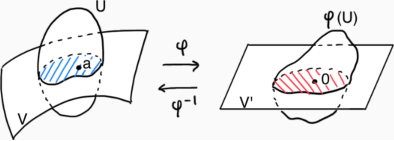
\includegraphics[width=0.5\textwidth]{figs/variete}
		\hfill
		\pause
		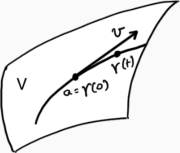
\includegraphics[width=0.2\textwidth]{figs/tangente}
	\end{figure}
	
	\item Un vecteur $v$ est \alert{tangent} à $V_g$ en $a$ s'il existe un chemin différentiable $\gamma:[0,1] \to \RR^n$ sur la variété tel que $\gamma(0) = a$ (\alert{$\gamma$ passe par $a$}) et $\gamma'(0) = v$ (\alert{$v$ est tangent au chemin en $a$}). 
	
	\pause
	
	\item L'ensemble des vecteurs tangents à une variété lisse en $a$ est un espace vectoriel, appelé \alert{espace tangent}. Dans notre cas,
	\eq{\tcbhighmath{
		\Tt_a(V_g) = \Spanf\left({\nabla g_1(a),\ldots,\nabla g_p(a)}\right)^\bot
	}}
	
\end{itemize}

\end{frame}



\begin{frame}
\frametitle{Conditions nécessaires d'optimalité}

\begin{itemize}[label=\tiny$\blacksquare$]
	\item Si $f$ atteint son minimum sur $V$ en $x_*$, alors pour tout chemin différentiable $\gamma : [0,1] \to \RR^n$ sur $V_g$ tel que $\gamma(t_*) = x_*$ on doit avoir
\eq{
	(f \circ \gamma)'(t_*) = \nabla f(x_*)^\top \gamma'(t_*) = 0.
}

\item Autrement dit, \alert{$\nabla f(x_*)$ est orthogonal à l'espace tangent de $V_g$ en $x_*$}, \ie ici
\vspace{-10pt}
\begin{columns}[t]
\begin{column}{0.4\textwidth}
	\begin{figure}
	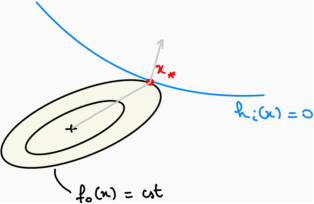
\includegraphics[width=0.7\textwidth]{optimalite-contraintes}
	\end{figure}
\end{column}
\begin{column}{0.6\textwidth}
\eq{
\begin{aligned}
	&\nabla f(\xx_*) \in \Spanf\left(\nabla g_1(\xx_*),\ldots,\nabla g_p(\xx_*)\right)\\
	\iff
	&\exists\, \nnu \in \RR^p, \;\, \nabla f(\xx_*) = -\sum\nu_{*i} \nabla g_i(\xx_*)\\
	\iff
	&\exists\, \nnu \in \RR^p, \;\, \nabla (f + \sum \nu_{*i} g_i)(\xx_*) = 0
\end{aligned}
}
\end{column}
\end{columns}


\item La fonction
\eq{\tcbhighmath{
	\Ll(\xx,\nnu) \eqdef f(\xx) + \sum_{i=1}^p \nu_i g_i (\xx)
}}
s'appelle le \alert{Lagrangien} du problème, les variables $\nu_i$ s'appellent des \alert{multiplicateurs de Lagrange}. Les CN d'optimalité du problème s'écrivent
\eq{\left\{
	\begin{aligned}
	&\nabla_{\xx} \Ll(\xx,\nnu) = 0 \quad\text{(ce qu'on vient de voir)}\\
	&\nabla_{\nnu} \Ll(\xx,\nnu) = 0 \quad\text{(on retrouve les contraintes d'égalités)}
	\end{aligned}
	\right.
}
\end{itemize}

\end{frame}


\begin{frame}
\frametitle{Cas général}

\begin{itemize}[label=\tiny$\blacksquare$]
	\item On considère un problème d'optimisation avec contraintes d'égalité et d'inégalité
	\eq{
		\min f(x) \qstq \left\{
		\begin{aligned}
			&g_i(\xx) = 0 \quad i=1,\ldots,p\\
			&h_j(\xx) \leq 0 \quad j=1,\ldots,q
		\end{aligned}\right.
	}
	où les fonctions $f$, $g_i$, $h_j$ sont \alert{convexes}, \alert{différentiables}
	
	\item A l'optimum, on a soit $h_j(\xx_*) < 0$ (\alert{contrainte inactive}), soit $h_j(\xx_*) = 0$ (\alert{contrainte active})
	
	
	\item On définit le \alert{Lagrangien} du problème
	\eq{\tcbhighmath{
		\Ll(\xx,\lla,\nnu) \eqdef f(\xx) + \sum_{i=1}^p \nu_i g_i(x) + \sum_{j=1}^q \la_j h_j(\xx)
	}}
	
	Les conditions nécessaires d'optimalité du problème (\alert{conditions KKT}) sont
	\eq{\left\{
		\begin{aligned}
			&\tcbhighmath[colback=blue!20,top=-2pt,bottom=-2pt]{\nabla_{\xx}\Ll(\xx,\lla,\nnu) = 0}\\
			&\tcbhighmath[colback=green!20,top=-2pt,bottom=-2pt]{g_i(\xx) = 0 \quad i=1,\ldots,p} \\
			&\tcbhighmath[colback=red!20,top=-2pt,bottom=-2pt]{\la_{j} \geq 0 \quad j=1,\ldots,q}\\
			&\tcbhighmath[colback=red!20,top=-2pt,bottom=-2pt]{\la_{j}h_j(\xx) = 0 \quad j=1,\ldots,q}
		\end{aligned}\right.
	}
	%\item A l'optimum $x_*$, on a soit $h_j(\xx_*) < 0$ (\alert{contrainte inactive}), soit $h_j(\xx_*) = 0$ (\alert{contrainte active}): cela se traduit sur le multiplicateur de Lagrange associé
		%\eq{
		%	\la_{*j} h_j(\xx_*) = 0
		%}
\end{itemize}
\end{frame}


\begin{frame}
\frametitle{Problème dual}

\begin{itemize}[label=\tiny$\blacksquare$]
\item \begin{thm}[Dualité forte] Sous certaines conditions non discutées ici, on a

\eq{
	\begin{aligned}
	&\min_{\xx} f(x) \qstq \left\{
		\begin{aligned}
			&g_i(\xx) = 0 \quad i=1,\ldots,p\\
			&h_j(\xx) \leq 0 \quad j=1,\ldots,q
		\end{aligned}\right.\\
	\iff
		&\min_{\xx}\max_{\lla \geq 0,\nnu} \Ll(\xx,\lla,\nnu)\\
	\iff
		&\max_{\lla \geq 0,\nnu}\min_{\xx} \Ll(\xx,\lla,\nnu) \defeq \tcbhighmath{\max_{\lla \geq 0,\nnu} d(\lla,\nnu)}
	\end{aligned}
}
\end{thm}

\item Le problème de maximisation s'appelle \alert{problème dual} (le problème initial, \alert{problème primal})

\item La minimisation par rapport à $\xx$ de $\Ll(\xx,\lla,\nnu)$ fait (souvent) apparaître des contraintes sur $\lla$ et/ou $\nnu$ (provenant de la condition $\nabla_{\xx} \Ll = 0$)
\end{itemize}

\end{frame}



\begin{frame}
\frametitle{Cas des SVM}

\begin{itemize}[label=\tiny$\blacksquare$]
	\item On souhaite résoudre le problème contraint:
	
	\eq{
		\min \frac{1}{2}\norm{\abold}^2 \qscq  y_j(\abold^\top \xx_j + b) \geq 1, \quad j=1,\ldots,q
	}

	\item C'es un problème \alert{convexe}. On considère le \alert{Lagrangien}
	\eq{\tcbhighmath{
		\Ll(\abold,b,\bm{\lla}) = \frac{1}{2}\norm{\abold}^2 + \sum_{j=1}^q\la_i(1-y_i(\abold^\top \xx_i + b))
	}}
	
	Les contraintes d'inégalités sont \alert{affines} en $(\abold,b)$: les conditions KKT sont aussi \alert{suffisantes} dans ce cas, et il y a \alert{dualité forte}!
	
	\eq{
	\left\{\begin{aligned}
			&\nabla_{\abold} \Ll(\abold,b,\lla) = 0 \iff \tcbhighmath{\abold = \sum \la_j y_j \xx_j}\\
			&\nabla_b \Ll(\abold,b,\lla) = 0 \iff \sum \la_jy_j = 0\\
			& \la_j \geq 0, \quad \la_j(1-y_j(\abold^\top \xx_i+b)) = 0 \quad \forall j \quad \tcbhighmath[colback=black!2]{\textcolor{black!2}{\sum}}
	\end{aligned}\right.
}
	
\end{itemize}
	
\end{frame}


\begin{frame}
\frametitle{SVM dual}

\begin{itemize}[label=\tiny$\blacksquare$]
	\item Injectées dans le Lagrangien, les relations précédentes conduisent au problème dual associé
	\eq{\tcbhighmath{\begin{aligned}
		\max_{\lla} \quad &\sum_{j=1}^q \la_j - \frac{1}{2}\sum_{j,j'=1}^q \la_j\la_{j'}y_jy_{j'}\xx_j^\top\xx_{j'} \\
		\qscq
			&\sum\la_j y_j = 0, \quad \la_j \geq 0, \quad j=1,\ldots,q
		\end{aligned}}
	}
	
	\item On préfère souvent résoudre cette formulation car elle ne dépend que des produits scalaires deux à deux des données $\xx_j^\top \xx_{j'}$
\end{itemize}
	

\end{frame}


\begin{frame}
\frametitle{Solution}

\begin{itemize}[label=\tiny$\blacksquare$]
	\item Le vecteur optimal $\abold_*$ normal à l'hyperplan séparateur est donné par
	\eq{
		\abold_* = \sum \la_{j*} y_j \xx_j
	}
	\item A l'optimum, les conditions KKT imposent
	$\la_{j*}(1-y_j(\abold_*^\top \xx_i+b)) = 0$:
	\begin{itemize}
	\item \alert{\textbf{1er cas}}:\; $y_j(\abold_*^\top \xx_i + b) > 1$
	
	\qquad Alors $\la_{j*} = 0$, et $\xx_j$ n'apparaît pas dans l'expression de $\abold$
	
	\item \alert{\textbf{2ème cas}}:\; $y_j(\abold_*^\top \xx_i + b) = 1$
	
	\qquad Alors $\la_{j*} \neq 0$, et $\xx_j$ se trouve sur la marge: c'est un \alert{vecteur de support}
	
	
\end{itemize}
\item La fonction de décision pour le problème de classification est finalement donnée par
	\eq{\tcbhighmath{
		\sgn\left(\sum_{j=1}^q\la_{j*}y_j \dotp{\xx}{\xx_j} + b_*\right)
	}}
\end{itemize}

\end{frame}



\section{SVM à marge souple}

\begin{frame}
\frametitle{Programme du cours}
\tableofcontents[currentsection]
\end{frame}


\begin{frame}
\frametitle{Limitations}

\begin{itemize}[label=\tiny$\blacksquare$]
	\item Une classification par hyperplan à marge dure n'est pas toujours souhaitable:
	\begin{itemize}[label=-]
		\item il peut y avoir des points aberrants/des erreurs dans les données: risque d'\alert{overfitting}
		\item les données ne sont pas toujours strictement linéairement séparables
	\end{itemize}
	
		
	\myfig{
		\onslide<1->{\includesvg[width=0.4\textwidth]{figs/exemples-lsvm-points-aberrants}}
		\onslide<2>{\includesvg[width=0.4\textwidth]{figs/exemples-lsvm-non-separables}}
	}
	
	\pause
	
	\item On voudrait autoriser les "mauvaises" classifications: on modifie la formulation du problème afin de \alert{pénaliser} les données mal classées
\end{itemize}

\end{frame}


\begin{frame}
\frametitle{SVM à marge souple}

\begin{itemize}[label=\tiny$\blacksquare$]
	\item meilleure robustesse aux données individuelles
	
	\item meilleure classification de \alert{la majorité} des données
	
	\item solution du problème d'optimisation
	\eq{
		\min \quad \frac{1}{2}\norm{a}^2 + \al \sum_{i=1}^p \xi_i
		\qscq y_i(\abold^\top \xx_i + b) \geq 1 - \xi_i, \quad \xi_i \geq 0, \quad i=1,\ldots,p
	}
	
	\item La contrainte
	\eq{
		y_i(\abold^\top \xx_i + b) \geq 1-\xi_i
	}
	autorise les échantillons du mauvais côté de la marge, voire de l'hyperplan, tandis que le terme $\al \sum \xi_i$ pénalise ces échantillons
	
	\item le paramètre $\al$ règle le compromis entre la largeur de la marge et le nombre d'échantillons mal classés
		\begin{itemize}[label=-]
			\item $\al$ grand: petite marge, moins d'erreurs de classification
			\item $\al$ faible: une grande marge, plus d'erreurs de classification 
		\end{itemize}
\end{itemize}
\end{frame}


\begin{frame}
\frametitle{Problème dual}

\begin{itemize}
	\item[1.] Calculer le Lagragien du problème SVM à marge souple
	\item[2.] Donner les conditions d'optimalité
	\item[3.] Formuler le problème dual
\end{itemize}
\end{frame}



\begin{frame}
\frametitle{Illustration}

\begin{figure}
	\captionsetup[subfigure]{labelformat=empty}
	\subfloat[$\al=0.02$]{\includesvg[width=0.25\textwidth]{figs/exemples-lsvm-soft-l0.02}}
	\quad
	\subfloat[$\al=0.07$]{\includesvg[width=0.25\textwidth]{figs/exemples-lsvm-soft-l0.07}}
	\\
	\subfloat[$\al=0.2$]{\includesvg[width=0.25\textwidth]{figs/exemples-lsvm-soft-l0.2}}
	\quad
	\subfloat[$\al=0.7$]{\includesvg[width=0.25\textwidth]{figs/exemples-lsvm-soft-l0.7}}
\end{figure}
\end{frame}


\section{Astuce du noyau}

\begin{frame}
\frametitle{Programme du cours}
\tableofcontents[currentsection]
\end{frame}


\begin{frame}
\frametitle{Cas non-linéaires}

Les données ne sont pas toujours linéairement séparables

\begin{figure}
	\includesvg[width=0.45\textwidth]{figs/exemples-nlsvm-dataset}
	\includesvg[width=0.45\textwidth]{figs/exemples-nlsvm-dataset-moons}
\end{figure}

\end{frame}


\begin{frame}
\frametitle{Transformation}

Les données peuvent devenir linéairement séparables après une \alert{transformation non-linéaire}
\eq{
	\mathbf{\phi} : \xx \mapsto \begin{bmatrix} \phi_1(\xx) & \phi_2(\xx) & \ldots \end{bmatrix} 
}



Exemple: $\phi$ transformation polynomiale
\begin{tikzpicture}
\node at (0,0) (ring) {\includesvg[width=0.4\textwidth]{figs/exemples-nlsvm-dataset}};
\node[right = 5em of ring] (lifted) {\includesvg[width=0.4\textwidth]{figs/exemples-nlsvm-dataset-lifted}};
\node[below = 3pt of lifted] (caption) {$\mathbf{\phi}(\xx) = \begin{bmatrix} x_1 & x_2 & x_1^2 + x_2^2 \end{bmatrix}$};

\draw[-latex] (ring.east) -- node[above]{$\phi$} (lifted.west);
\end{tikzpicture}
\end{frame}


\begin{frame}
\frametitle{Support Vector Machine}


\begin{itemize}[label=\tiny$\blacksquare$]
	\item Problème primal
	\eq{\tcbhighmath{
		\min \frac{1}{2}\norm{\abold}^2 + \al\sum_{j=1}^q \xi_j \qscq  y_i(\abold^\top \mathbf{\alert{\phi}}(\xx_j) + b) \geq 1 - \xi_j, \quad \xi_j \geq 0, \quad j=1,\ldots,q
	}}
	
	\item Problème dual
		\eq{\tcbhighmath{\begin{aligned}
		\max_{\lla} \quad &\sum_{j=1}^q \la_j - \frac{1}{2}\sum_{j,j'=1}^q \la_j\la_{j'}y_jy_{j'}\dotp{\alert{\phi}(\xx_j)}{\alert{\phi}(\xx_{j'})}\\
		\qscq
			&\sum\la_j y_j = 0, \quad \al \geq \la_j \geq 0, \quad j=1,\ldots,q
		\end{aligned}}
	}
	
	\item La fonction de décsision est finalement donnée par
	
	\eq{\tcbhighmath{
		\sgn\left(\sum_{j=1}^q\la_{j*}y_j \dotp{\phi(\xx)}{\phi(\xx_j)} + b_*\right)
	}}
\end{itemize}


\end{frame}


\begin{frame}
\frametitle{Le coup du noyau}

\begin{itemize}[label=\tiny$\blacksquare$]
	\item L'enjeu est de définir un noyau $K(\xx_j,\xx_{j'}) = \dotp{\phi(\xx_j)}{(\xx_{j'})}$ (un noyau est simplement une fonction symétrique de $\Xx \times \Xx$ dans $\RR$) tel que
	\begin{itemize}[label=-]
		\item la fonction de décision associée soit performante
		\item calculer $K(\xx_j,\xx_{j'})$ soit peu coûteux même en grande dimension
	\end{itemize}
		
	\item Exemples de noyaux
	\vfill
	\begin{center}
	\begin{tabular}{c|c}
		Polynomial de degré $d$ & $(1 + \dotp{\xx}{\xx'})^d$\\
		\hline
		Sigmoidal & $1/\eta_0 \tanh\left(\beta_0\dotp{\xx}{\xx'}+\al_0\right)$\\
		\hline 
		\hline
		Gaussien & $1/\eta_0 \exp\left(-\norm{\xx-\xx'}^2/\beta_0^2\right)$\\
		\hline
		Laplacien & $1/\eta_0 \exp\left(-\norm{\xx-\xx'}_1/\beta_0\right)$\\
		\hline
		Cauchy & $\frac{1}{\eta_0} \frac{1}{1+\norm{\xx-\xx'}^2/\beta_0^2}$
	\end{tabular}
	\end{center}
	
	\item Remarque: tout algorithme pouvant s'exprimer en termes de produits scalaires peut bénéficier de l'astuce du noyau
\end{itemize}
	
\end{frame}






%\bibliographystyle{apalike}
%\printbibliography
%\bibliography{/export/home/pcatala/Workspace/build/biblio}

\end{document}
